\section{Лекция 9}

\begin{definition}[Ранг типа]
$R(x)$ --- все типы ранга $x$.
\begin{itemize}
    \item $R(0)$ --- все типы без кванторов
    \item $R(x + 1) = R(x)\ |\ R(x) \rightarrow R(x + 1)\ |\ \forall \alpha.R(x + 1)$
\end{itemize}
\end{definition}

Например:
\begin{paracol}{2}
\begin{itemize}
    \item $\alpha \in R(0)$
    \item $\forall \alpha.\alpha \in R(1)$
    \item $(\forall \alpha.\alpha) \rightarrow (\forall b.b) \in R(2)$ 
    \item $((\forall \alpha.\alpha) \rightarrow (\forall b.b)) \rightarrow b \in R(3)$
\end{itemize}
\switchcolumn
Тут видно, если выражение слева от знака импликации имеет ранг $n$, то все выражение будет иметь ранг $\geq (n + 1)$.
\end{paracol}

\textbf{Утверждение}: Пусть $x$ --- выражение только с поверхностными кванторами, тогда $x \in R(1)$. 

\begin{definition}[Типовая схема]\

$\sigma ::= \forall \alpha_1. \forall \alpha_2. \dots \forall \alpha_n. \tau$, где $\tau \in R(0)$ и, следовательно, $\sigma \in R(1)$.

\end{definition}

\begin{definition}[Частный случай (специализация) типовой схемы]\

$\sigma_1, \sigma_2$ --- типовые схемы

$\sigma_2$ --- частный случай $\sigma_1$ (обознается как $\sigma_1 \sqsubseteq \sigma_2$), если 

\begin{enumerate}
    \item $\sigma_1 =  \forall \alpha_1. \forall \alpha_2. \dots \forall \alpha_n. \tau_1$
    \item $\sigma_2 =  \forall \beta_1. \forall \beta_2. \dots \forall \beta_m. \tau_1[\alpha_i := S(\alpha_i)]$
    \item $\forall i. \beta_i \in FV(\tau_1)$
\end{enumerate}

\end{definition}

\begin{example}\
	
$\forall \alpha . \alpha \rightarrow \alpha 
\sqsubseteq 
\forall \beta_1.\forall \beta_2: (\beta_1 \rightarrow \beta_2) \rightarrow (\beta_1 \rightarrow \beta_2)$

Вполне возможно, что в ходе замены, все типы будут уточнены ($\alpha$ уточнится как $\beta_1 \rightarrow \beta_2$.
\end{example}


\subsection{Хиндли-Милнер}

\begin{enumerate}
    \item Все типы только с поверхностными кванторами ($R(1)$)
    \item $\overline{HM} ::= p\ |\ \overline{HM}\ \overline{HM}\ |\ \lambda p. \overline{HM}\ |\ let =  \overline{HM}\ in\ \overline{HM}$
\end{enumerate}

\begin{itemize}
    \item $\exists p.\phi = \forall b.(\forall p. (\phi \rightarrow b)) \rightarrow b$
    \item $\phi \rightarrow \bot \equiv \forall b. (\phi \rightarrow b)$
    
    \item $\vcenter{\infer[]{\Gamma \vdash \forall b.(\forall p.(\phi \rightarrow b)) \rightarrow b}{\infer{\Gamma \vdash (\forall p. (\phi \rightarrow b)) \rightarrow b}{\infer{\Gamma, \forall p. (\phi \rightarrow b) \vdash b}{\infer{\Gamma, \forall p. (\phi \rightarrow b) \vdash \phi [p := \Theta] \rightarrow b}{\Gamma, \forall p. (\phi \rightarrow b) \vdash \forall p.(\phi \rightarrow b)}}}}}$
    % \item $\Gamma, \forall p. (\phi \rightarrow b) \vdash \forall p.(\phi \rightarrow b)$
    % \item $\Gamma, \forall p. (\phi \rightarrow b) \vdash \phi [p := \Theta] \rightarrow b$
    % \item $\Gamma, \forall p. (\phi \rightarrow b) \vdash b$
    % \item $\Gamma \vdash (\forall p. (\phi \rightarrow b)) \rightarrow b$
    % \item $\Gamma \vdash \forall b.(\forall p.(\phi \rightarrow b)) \rightarrow b$
\end{itemize}

Соглашение:
\begin{itemize}
    \item $\sigma$ --- типовая схема
    \item $\tau$ --- простой тип
\end{itemize}


\begin{enumerate}
    \item $\vcenter{\infer{\Gamma, x : \sigma \vdash x : \sigma}{}}$
    \item $\vcenter{\infer{\Gamma \vdash e_0\ e_1 : \tau'}{\Gamma \vdash e_0 : \tau \rightarrow \tau' \qquad \Gamma \vdash e_1 : \tau}}$
    \item $\vcenter{\infer{\Gamma \vdash \lambda x.e : \tau \rightarrow \tau'}{\Gamma, x : \tau \vdash e : \tau'}}$
    \item $\vcenter{\infer[,\ let\ x = a\ in\ b \equiv (\lambda x.b)\ a]{\Gamma \vdash let\ x = e_0\ in\ e_1 : \tau}{\Gamma \vdash e_0 : \sigma \qquad \Gamma, x : \sigma \vdash e_1 : \tau}}$ 
    \item $\vcenter{\infer{\Gamma \vdash e : \sigma}{\Gamma \vdash e : \sigma' \qquad  \sigma' \sqsubseteq \sigma}}$
    \item $\vcenter{\infer[\alpha \not \in FV(\Gamma)]{\Gamma \vdash e : \forall \alpha.\sigma}{\Gamma \vdash e : \sigma}}$
\end{enumerate}


\subsection{Алгоритм вывода типов в системе Хиндли-Милнера W}
На вход подаются $\Gamma,\ M$, на выходе наиболее общая пара $(S, \tau)$
\begin{enumerate}
    \item $M = x ,\ x:\tau  \in \Gamma$ (иначе ошибка)
    \begin{itemize}
        \item Выбросить все кванторы из $\tau$
        \item Переименовать все свободные переменные в свежие \\
        Например: $\forall \alpha_1.\phi \Rightarrow \phi[\alpha_1 := \beta_1]$, где $\beta_1$ --- свежая переменная
    \end{itemize}
    $(\emptyset, \Gamma(x))$
    \item $M = \lambda n.e$
    \begin{itemize}
        \item $\tau$ --- новая типовая переменная
        \item $\Gamma' = \Gamma \setminus \{n : \_ \}$ (т.е. $\Gamma$ без переменной $n$)
        \item $\Gamma'' = \Gamma' \cup {n : \tau}$
        \item $(S',\ \tau') = W(\Gamma'', e)$
    \end{itemize}
    $(S', S'(\tau) \rightarrow \tau')$
    \item $M = P\ Q$
    \begin{itemize}
        \item $(S_1, \tau_1) = W(\Gamma, P)$
        \item $(S_2, \tau_2) = W(S_1(\Gamma), Q)$
        \item $S_3$ --- Унификация $(S_2(\tau_1), \tau_2 \rightarrow \tau)$
    \end{itemize}
    $(S_3 \circ S_2 \circ S_1, S_3(\tau))$
    \item $let\ x = P\ in\ Q$
    \begin{itemize}
        \item $(S_1, \tau_1) = W(\Gamma, P)$
        \item $\Gamma' = \Gamma$ без $x$
        \item $\Gamma'' = \Gamma' \cup \{ x : \forall \alpha_1 \dots \alpha_k. \tau_1 \}$, где $\alpha_1 \dots \alpha_k$ все свободные переменные в $\tau_1$
        \item $(S_2, \tau_2) = W(S_1(\Gamma''), Q)$
    \end{itemize}
    $(S_2 \circ S_1), \tau_2)$
\end{enumerate}

Надеемся, что логика второго порядка противоречива. \\

\subsection{Рекурсивные типы}

Ранее мы уже рассматривали $Y$-комбинатор, но не могли типизировать его и отказывались. 
Однако в программировании хотелось бы использовать рекурсию, поэтому тут мы введем его аксиоматически.

$Y f =_\beta f (Y\ f)$

$Y : \forall \alpha . (\alpha \rightarrow \alpha) \rightarrow \alpha$ --- аксиома

И теперь, когда мы хотим написать какую-то рекурсивную функцию, скажем, на языке Ocaml, то интерпретировать ее можно будет следующим образом:

\begin{paracol}{2}
\begin{minted}[escapeinside=||,mathescape=true]{fsharp}
let rec f = expr in
    expression
\end{minted}
\switchcolumn
\begin{minted}[escapeinside=||,mathescape=true]{fsharp}
let f = Y (|$\lambda$| f. expr) in
    expression
\end{minted}
\end{paracol}

Рекурсивными могут быть не только функции, но и типы. Как, например, список из целых чисел:

\begin{minted}{fsharp}
type intList = Nil | Cons of int * intList;;
\end{minted}

На нем мы можем вызывать рекурсивные функции, например, ниже представлен фрагмент кода, позволяющий найти длину списка. 

\begin{minted}{fsharp}

let rec length l = match l with 
  | Nil -> 0
  | Cons (x, s) -> 1 + length s;;

let my_list = Cons(1, Cons (2, Cons (3, Nil)));;

print_int (length my_list);;  (* output: 3 *)
\end{minted}

Рассмотрим, что из себя представляет тип списка выше:


$Nil = inLeft\ O = \lambda a. \lambda b. a\ O$ 

$Cons = inRight\ p = \lambda a. \lambda b. b\ p$

$\lambda a. \lambda b. a\ O : \forall \gamma .(\alpha \rightarrow \gamma) \rightarrow (\beta \rightarrow \gamma) \rightarrow \gamma$

$\lambda a. \lambda b. b\ O: \forall \gamma .(\alpha \rightarrow \gamma) \rightarrow (\beta \rightarrow \gamma) \rightarrow \gamma$

$\delta = \forall \gamma .(\alpha \rightarrow \gamma) \rightarrow (\beta \rightarrow \gamma) \rightarrow \gamma$

$\lambda a. \lambda b. b\ (\lambda a. \lambda b. a\ O) : \forall \alpha. (\alpha \rightarrow \gamma) \rightarrow (\delta \rightarrow \gamma) \rightarrow \gamma$


\vspace{5mm}
Научимся задавать рекурсивные типы, а именно рассмотрим два способа решения:

\begin{enumerate}
    \item Эквирекурсивный 
    \begin{minted}{fsharp}
        list = Nil | Cons a * list
    \end{minted}
    $\alpha = f(\alpha)$ --- уравнение с неподвижной точкой. Пусть $\mu \alpha. f(\alpha) = f(\mu \alpha.f(\alpha))$. Используем это в типах, а именно $f$ - это и тип список. То есть мы по сути использовали $Y$ комбинатор, который для выражений, а для типов ввели аналогичный $\nu$.
    
    На практике такой подход используется и в языке программирования Java:
    
    \begin{minted}{java}
        class Enum <extends Enum<E>>
    \end{minted}
    
    Также приведем пример вывода типа $\lambda x. x\ x$ (можно вспомнить, что именно этот терм помешал нам типизировать $Y$-комбинатор в просто типизированном $\lambda$-исчислении): 
    
    \begin{paracol}{2}
    \switchcolumn
            $\vcenter{\infer{\vdash \lambda x. x\ x : \tau \rightarrow \beta}{\infer[]{x : \tau \vdash x\ x : \beta}{x : \tau \vdash x : \tau \rightarrow \beta \qquad x : \tau \vdash x : \tau}}}$
    \switchcolumn
        Пусть $\tau = \mu \alpha. \alpha \rightarrow \beta$. Если мы раскроем $\tau$ один раз, то получим $\tau = \tau \rightarrow \beta$. Если раскроем еще раз, то получим $\tau = (\tau \rightarrow \beta) \rightarrow \beta$.
    \end{paracol}
    
    Ранее мы ввели $Y$-комбинатор аксиоматически, а можем ли мы его типизировать используя рекурсивные типы? Ответ: Да, можем. Напомним, что $Y = \lambda f.(\lambda x. f\ (x\ x))\ (\lambda x. f\ (x\ x))$.
    
    $\vcenter{\infer[]{\vdash \lambda f.(\lambda x. f\ (x\ x))\ (\lambda x. f\ (x\ x)) : \forall \beta. (\beta \rightarrow \beta) \rightarrow \beta}{\infer[]{\vdash \lambda f.(\lambda x. f\ (x\ x))\ (\lambda x. f\ (x\ x)) : (\beta \rightarrow \beta) \rightarrow \beta}{\infer[]{f : \beta \rightarrow \beta \vdash (\lambda x. f\ (x\ x))\ (\lambda x. f\ (x\ x)) : \beta}{\infer {\lambda f : \beta \rightarrow \beta \vdash \lambda x. f\ (x\ x) : \tau \rightarrow \beta}{\infer[]{f : \beta \rightarrow \beta \vdash \lambda x. f\ (x\ x) : \tau}{\infer[]{f : \beta \rightarrow \beta, x : \tau \vdash f\ (x\ x)}{\lambda f : \beta \rightarrow \beta,\ x : \tau \vdash f : \beta \rightarrow \beta \qquad f : \beta \rightarrow \beta,\ x : \tau \vdash x\ x : \beta}}} \qquad \infer{\lambda f : \beta \rightarrow \beta \vdash \lambda x. f\ (x\ x) : \tau}{\text{аналогично в другой ветке}}}}}}$
    
    Загадочка: А можно ли типизировать, скажем $\lambda x : Nat. x (S x)$?
    \item Изорекурсивный
    
    В отличие от эквирекурсивных типов будем считать, что $\mu \alpha. f(\alpha)$ изоморфно $f(\mu \alpha.f(\alpha))$. Такой подход используется в языке программирования C.
    \begin{minted}{C}
    struct list {
        list* x;
        int a;
    }
    (*x).(*x).(*x).a
    // или, что эквивалентно
    x->x->x.a
    \end{minted}
    
    Можно заметить, что выше для работы со списком мы использовали специальную операцию:
    $*: list* \rightarrow list$ --- разыменование 
    
    В изорекурсивных типах введены специальные операции для работы с этими типами, и оператор * из C как раз был примером одной из них (в частности roll):
    \begin{itemize}
        \item $Roll: Nil | Cons (a * list) \rightarrow list$
        \item $Unroll: list \rightarrow Nil | Cons (a * list)$
    \end{itemize}
    
    В более общем виде (введение в типовую систему): 
    \begin{itemize}
        \item $roll: f(\alpha) \rightarrow \alpha$
        \item $unroll: \alpha \rightarrow f(\alpha)$
    \end{itemize}
    
    Можно привести еще примеры из языка C:
    \begin{itemize}
        \item $*: T* \rightarrow T$
        \item $\&: T \rightarrow T*$
        \item $T = \alpha$
        \item $T* = f(\alpha)$
    \end{itemize}
    
\end{enumerate}

\subsection{Зависимые типы}
    
Рассмотрим функцию sprintf из языка C:
    
    $sprintf : string \rightarrow smth \rightarrow string$
    
    $sprintf "\%d" : int \rightarrow string$
    
    $sprintf "\%f" : float \rightarrow string$
    
Легко видеть, что тип sprintf определяется первым аргументом. То есть тип этой функции зависит от терма — именно такой тип и называется зависимым (\textit{англ: dependent type}). 

Рассмотрим несколько иной пример, а именно список. Предположим, что мы хотим скалярно перемножить два списка: 

\begin{minted}{fsharp}
let rec dot lst1 lst2 = match (lst1, lst2) with
  | ([], []) -> 0
  | (x :: xs, y :: ys) -> x * y + (dot xs ys)
;;

dot [1; 2] [3; 4] (* results in 11 *)

dot [1; 2] [3; 4; 5] (* получим ошибку *)

\end{minted}

Было бы очень здорово уметь отлавливать эту ошибку не в рантайме, а во время компиляции программы и зависимые типы могут в этом помочь. Например в языке Idris можно использовать Vect: 

\begin{minted}{fsharp}
dot : {n : Nat} -> Vect n Integer -> Vect n Integer -> Integer
dot {n = Z} [] [] = 0
dot {n = (S len)} (x :: xs) (y :: ys) = y * x + dot xs ys 

let v1 = Data.Vect.fromList [1, 2, 3]
let v2 = Data.Vect.fromList [4, 5, 6]
dot v1 v2 -- results in 32

let v1 = Data.Vect.fromList [1, 2, 3, 4]
dot v1 v2 -- Type mismatch between
          --      Vect 3 Integer (Type of v2)
          -- and
          --      Vect 4 Integer (Expected type)
\end{minted}

Если подойти к типу функции dot ближе с точки зрения теории типов, то мы бы записали это так (о * речь пойдет в следующей главе [стоит ее воспринимать как тип типа]):

$Nat : *,\ Integer : *,\ Vect : Nat \rightarrow Integer \rightarrow * \vdash dot : \Pi n : Nat. (Vect\ n\ Integer) \rightarrow (Vect\ n\ Integer) \rightarrow Integer$

\subsubsection{$\Pi$-типы и $\Sigma$-типы}

\begin{itemize}
    \item $\Pi x : \alpha . P(x)$ - эту запись можно читать как (в каком-то смысле в интуиционистском понимании): "У меня есть метод для конструирования объекта типа $P(x)$, использующий любой предоставленный $x$ типа $\alpha$". Если же смотреть на эту запись с точки зрения классической логики, то ее можно понимать как бесконечную  конъюнкцию $P(x_1)\&P(x_2)\&...$. Данная конъюнкция соответствует декартовому произведению, отсюда и название $\Pi$-типа (иногда в англоязычной литературе можно встретить \textit{dependent function type}).
    \item $\Sigma x : \alpha . P(x)$. Аналогично предыдущему пункту рассмотрим значение с интуиционистской точки зрения: "У меня есть объект $x$ типа $\alpha$, но больше ничего про него не знаю кроме того, что он обладает свойством $P(x)$". Это как раз в стиле интуиционизма, что нам приходится знать и объект $x$ и его свойство $P(x)$. Это можно представить как пару, а пара - бинарное произведение. С точки же зрения классической логики, мы можем принимать эту формулу как бесконечную дизъюнкцию $P(x_1) \vee P(x_2)\vee ...$, которая соответствует алгебраическим типам данных. (иногда в англоязычной литературе можно встретить \textit{dependent sum}).
\end{itemize}

Ранее обсуждалось, что тип может быть сопоставлен множеству его значений, как например тип uint32\_t в С++ может быть сопоставлен множеству $\{0, 1, ..., 2^{32} - 1\}$. Рассмотрим $\Pi x : \alpha . P(x)$: этому $\Pi$-типу можно сопоставить прямое произведение $B^A$ (где $A$ --- множество, сопоставленное типу $\alpha$, а $B(a)$ - множество, сопоставленное типу $P(a)$), которое следует воспринимать, как $B^A = \prod_{a \in A} B(a) = \{ f : A \rightarrow \bigcup_{a \in A} B(a)\ |\ f(a) \in B(a), a \in A  \}$. Можно отметить, что если $B(a) = C = const$, то на любой вход $f(a) \in C$, т.е. тип значения $f(a)$ не меняется, собственно поэтому этот тип в таком случае записывают как $A \rightarrow P$. Рассмотрим $\Sigma x : \alpha . P(x)$: этому $\Sigma$-типу можно сопоставить дизъюнктное объединение $\sqcup_{a \in A} B(a) = \bigcup_{a \in A}\{(a, x) | x \in B(a)\}$, где $A$ --- множество, сопоставленное типу $\alpha$, а $B(a)$ - множество, сопоставленное типу $P(a)$. Тут также можно отметить, что если $B(a) = C = const$, то результатом дизъюнктивного объединения будет прямое произведение $A \times B$. В языке программирования Idris примером $\Sigma$-типа является зависимая пара:

\begin{minted}{fsharp}
data DPair : (a : Type) -> (P : a -> Type) -> Type where
  MkDPair : {P : a -> Type} -> (x : a) -> P x -> DPair a P
\end{minted}

Также есть некоторый синтаксический сахар (a : A ** P), который обозначает зависимую пару типа DPair A P, где P может содержать в себе имя a.

В документации Idris'а есть хороший пример использования: мы хотим отфильтровать вектор  (Vect) по какому-то предикату - мы не можем знать заранее длину результирующего вектора, поэтому зависимая пара выручает:

\begin{minted}{fsharp}
filter : (a -> Bool) -> Vect n a -> (p ** Vect p a)
filter p Nil = (_ ** [])
filter p (x :: xs) with (filter p xs)
  | ( _ ** _xs ) = if (p x) then 
                    ( _ ** x :: _xs ) 
                  else 
                    ( _ ** _xs )
\end{minted}


\section{Лекция 10}

\subsection{Введение}

Прежде мы разбирали просто типизированное лямбда-исчисление, в котором термы зависели от термов, например, терм $(F\ M)$ зависит от терма $M$. После того, как было замечено, что, скажем, I может иметь разные типы, которые по сути различаются лишь аннотацией, например, $\lambda x. x : \alpha \rightarrow \alpha$, $\lambda x. x : (\alpha \rightarrow \alpha) \rightarrow (\alpha \rightarrow \alpha)$, была введена типовая абстракция, то есть термы теперь могли зависеть от типов и такая типовая система была названа System F и можно было писать $\Lambda \alpha. \lambda x : \alpha . x : \forall \alpha. \alpha \rightarrow \alpha$. То есть это было своего рода изобретением шаблонов в языке C++. Но на этом все не ограничено. System $F_w$, в которой типы могут зависеть от типов, как, например, список - алгебраический тип данных, у которого есть две альтернативы $Nil : \forall \alpha . List \alpha$ и $Cons : \forall \alpha. \alpha \rightarrow List \alpha \rightarrow \alpha$ (рекурсивные типы смотри выше). Для лучшего понимания различия системы $F$ и $F_w$ ниже представлены грамматики для типов:
\begin{itemize}
    \item $T_\rightarrow ::= \alpha\ |\ (T_\rightarrow)\ |\ T_\rightarrow \rightarrow T_\rightarrow$
    \item $T_F ::= \alpha\ |\ \forall \alpha. T_F\ |\ (T_F)\ |\ T_F \rightarrow T_F$ 
    \item $T_{F_w} ::= \alpha\ |\ \lambda \alpha. T_{F_w}\ |\ (T_{F_w})\ |\ T_{F_w} \rightarrow T_{F_w}\ |\ T_{F_w}\ T_{F_w} $
\end{itemize}

Ничего не мешает рассматривать типовую систему, в которой тип может зависеть от терма, как это было сделано раньше. Пусть для всех $a : \alpha$ мы можем определить тип $\beta_\alpha$ и пусть существует $b_\alpha : \beta_\alpha$. Тогда вполне обоснована запись функции $\lambda \alpha : b_\alpha$. Тип данного выражения принято записывать как $\Pi a :\alpha . \beta_\alpha$ (стоит сделать замечание, что если $\beta_\alpha$ не зависит от $\alpha$ [то есть функция константа], то вместо $\Pi a :\alpha . \beta_\alpha$ пишут $\alpha \rightarrow \beta$). Примером может быть тип вектора, длина которого зависит от натурального числа и типа (пример из языка Idris):
\begin{minted}{Fsharp}
data Vect : (len : Nat) -> (elem : Type) -> Type where
  Nil  : Vect Z elem
 (::) : (x : elem) -> (xs : Vect len elem) -> Vect (S len) elem
\end{minted}

Теперь наша грамматика стала обширной и появилась необходимость более формально говорить о типах, т.е. ввести их в систему. Для этого был придуман род (\textit{англ: kind}), который обозначают $*$. Используя $*$ можно задавать типы типовых конструкторов. 

Рассмотрим пару примеров, как используется род:

\begin{itemize}
    \item $\lambda m : \alpha.F\ m : (\alpha \rightarrow \beta) : *$
    \item $\lambda \alpha : *.I_\alpha : (\Pi \alpha : * . \alpha \rightarrow \alpha):*$
    \item $\lambda n : Nat . A^n \rightarrow B : Nat \rightarrow *$
    \item $\lambda a : *. a \rightarrow a : * \rightarrow *$
\end{itemize}

Попробуем разобраться, что же написано в примерах. 

\begin{itemize}

    \item Первый пример - это типизация привычной нам абстракции. Утверждение $a \rightarrow b : *$ значит $a \rightarrow b$ - это тип. 

    \item Во втором примере мы рассматриваем лямбда-выражение, которое принимает на вход тип и возвращает терм $I_\alpha$. Таким образом мы собираемся типизировать терм, зависящий от типа. Для этого как сказано выше мы вводим символ $\Pi$, а вот в известной нам системе F тип выражения $\lambda \alpha : *.I_\alpha$ был бы $\forall \alpha. (\alpha \rightarrow \alpha)$.

    \item В третьем пункте мы хотим сформировать утверждения для типа, зависящего от терма. Интуитивно понятно, что у такого выражения будет род $Nat \rightarrow *$. И заселять его будут конструкторы типов, которые принимают на вход число и возвращают тип, например $\lambda x : Nat. int [x]$ - это терм, который заселяет род  $Nat \rightarrow *$

    \item В четвертом пункте мы типизируем конструктор типа, который принимает на вход тип. Действительно, его родом будет $* \rightarrow *$.

\end{itemize}

Возникает желание каким-то образом объединить все роды, и это необходимо для дальнейшей формализации происходящего. $* \rightarrow * : ?$. Что можно поставить на место вопросика? Это не тип, так как иначе бы могли записать $* \rightarrow * : *$, однако понятно, что это не так. В частности для этого вводится понятие сорта (\textit{англ. sort}), которое можно воспринимать как тип рода и тогда $* \rightarrow * : \openbox $ и $* : \openbox$. Для любого выражения вида $A \rightarrow *$, где A - это что угодно, верно, что оно типизируется $\openbox$. Например,

$* \rightarrow * \rightarrow * : \openbox$ - этот род очень похож на $* \rightarrow *$, и действительно, единственное отличие заключается в количестве аргументов нашего типового конструктора. В частности, этот род заселяет конструктор map, $\lambda keyType : *. (\lambda valueType. map<keyType, valueType>)$
    
Теперь мы ознакомились со всеми необходимыми обозначениями и неформальными определениями. Обобщая все вышесказанное, построим обобщенную типовую систему.

\subsection{Обобщенная типовая система}
\begin{itemize}
    
\item Сорта: \{*, \openbox\}
\begin{itemize}
    \item Выражение "$A:*$" означает, что $A$ --- тип. И тогда, если на метаязыке мы хотим сказать "Если $A$ тип, то и $A \rightarrow A$ тоже тип", то формально это выглядит как $A:* \vdash (A \rightarrow A):*$
    \item $\openbox$ - это абстракция над сортом для типов.
    \item Например:
    \begin{itemize}[leftmargin = 2cm]
        \item $5:int:*:\openbox$
        \item $[]:*\rightarrow*:\openbox$
        \item $\Lambda M.List<M>:*\rightarrow* : \openbox$
    \end{itemize}
\end{itemize}

\item $T ::= x\ |\ c\ |\ T\ T\ |\ \lambda x:T.\ T\ | \Pi x:T.\ T$

\item Аксиома:
\begin{itemize}
    \item $\vcenter{\infer{\vdash * . \openbox}{}}$
\end{itemize}

\item Правила вывода:
\begin{enumerate}
    \item $\vcenter{\infer[x \not \in \Gamma]{\Gamma, x : A \vdash x : A}{\Gamma \vdash A:S}}$
    \item $\vcenter{\infer[\text{--- правило ослабления (примерно как } \alpha \rightarrow \beta \rightarrow \alpha \text{ в И.В.)}]{\Gamma, x : C \vdash A:B}{\Gamma \vdash A:B \qquad \Gamma \vdash C:S}}$
    \item $\vcenter{\infer[\text{--- правило конверсии}]{\Gamma \vdash A:B'}{\Gamma \vdash A:B \qquad \Gamma \vdash B':S \qquad B =_\beta B'}}$
    \item $\vcenter{\infer[\text{--- правило применения}]{\Gamma \vdash (F\ a) : B[x := a]}{\Gamma \vdash F : (\Pi x:A.B) \qquad \Gamma \vdash a : A}}$
\end{enumerate}

\item Семейства правила (generic-правила)

Пусть $(s_1, s_2) \in S \subseteq \{*, \openbox\}^2$.

\begin{enumerate}
    \item $\Pi$-правило: $\vcenter{\infer[]{\Gamma \vdash (\Pi x : A.B) : s_2}{\Gamma \vdash A : s_1 \qquad \Gamma, x : A \vdash B : s_2}}$
    \item $\lambda$-правило: $\vcenter{\infer[]{\Gamma \vdash (\lambda x : A . b) : (\Pi x : A. B)}{\Gamma \vdash A:s_1 \qquad \Gamma, x : A \vdash b : B \qquad \Gamma, x : A \vdash B : s_2}}$
\end{enumerate}

\end{itemize}

В одном из примеров мы рассмотрели утверждение $\lambda \alpha : *.I_\alpha : (\Pi \alpha : * . \alpha \rightarrow \alpha):*$. Теперь мы можем до конца понять, почему $(\Pi \alpha : * . \alpha \rightarrow \alpha):*$ и что такое $\Pi$. Неформально говоря, $\Pi$-правило говорит нам о том, что выражение $(\Pi x : A.B)$ типизируется либо $*$, либо $\openbox$, а именно тем, чем является B. То есть, $(\Pi x : A.B)$ - это либо тип конструктора типа, либо тип конструктора терма. В приведенном примере мы принимаем на вход любой тип $\alpha$  и возвращаем терм, а значит $(\Pi \alpha : * . \alpha \rightarrow \alpha):*$.

Еще пару слов про $\Pi$. Этот символ является обобщением $\rightarrow$, поэтому, во всех рассмотренных ранее родах, согласно нашей обобщенной типовой системе, можно заменить $\rightarrow$ на $\Pi$, согласно замечанию выше. Например, $* \rightarrow * = \Pi a : *. *$. Важно понимать, что подразумевается под зависимостью тела от аргумента и не путать понятия терм и тип. В $\Pi a : *. *$ тело не зависит от аргумента, потому что тело - это просто звездочка, то есть  $\Pi a : *. *$ говорит нам просто о том, что наше выражение принимает тип и выдает тип. В то время как термы, населяющие $\Pi a : *. *$, разумеется, могут иметь тело, зависящее от аргумента, как, например, $\lambda a : *. a \rightarrow a$

\subsection{$\lambda$-куб}

В обобщенных типовых системах есть generic-правила, которые зависят от выбора $s_1$ и $s_2$ из множества сортов. Этот выбор можно проиллюстрировать в виде куба.

\begin{center}
    {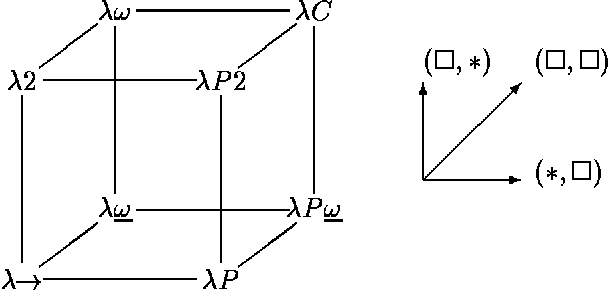
\includegraphics[scale=0.5]{pic.png}}
\end{center}

Выбор правил означает следующее:
\begin{itemize}
    \item $(*,\ *)$ - позволяет записывать термы, которые зависят от термов
    \item $(\openbox,\ *)$ - позволяет записывать термы, которые зависят от типов
    \item $(*,\ \openbox)$ - позволяет записывать типы, которые зависят от термов
    \item $(\openbox,\ \openbox)$ - позволяет записывать типы, которые зависят от типов
\end{itemize}

На самом деле в данной формулировке под типом понимается не только привычный тип. Потому что для привычного типа верно $\tau : *$. Здесь же $\tau$ может типизироваться чем угодно, кроме $\openbox$. В частности $* \rightarrow *$, это значит, что 
    
Также на этом кубике можно расположить языки программирования, например:
\begin{itemize}
    \item Haskell будет располагаться на левой грани куба, недалеко от $\lambda w$
    \item Idris и Coq, очевидно, будет находиться в $\lambda C$
    \item C++ очень ограниченно приближается к $\lambda C$ (мысли вслух):
    \begin{enumerate}
        \item $(*,\ *)$ - без этого не может обойтись ни один язык программирования
        \item $(\openbox,\ *)$ - например, sizeof(type)
        \item $(*,\ \openbox)$ - например, std::array<int, 19> - тут есть ограничение на то, значение каких типов можно подставлять.
        \item $(\openbox,\ \openbox)$ - например, std::vector<int>, int*
    \end{enumerate}
\end{itemize}

\subsection{Свойства}

Для систем в $\lambda$-кубе верны следующие утверждения:
\begin{itemize}
    \item \textbf{Th. SN} \qquad \qquad \qquad \quad \quad \ Обобщенная типовая система сильно нормализуема
    \item \textbf{Th. Черча-Россера} \quad \begin{minipage}{0.6\textwidth}
\raggedright % obviates the need for explicit linebreaks
\begin{enumerate}
    \item Для любых трёх элементов $A$, $B$ и $C$, таких, 
    $A \twoheadrightarrow B$ и $A \twoheadrightarrow C$ верно,
    что существует $D$, что 
    $B \twoheadrightarrow D$ и $C \twoheadrightarrow D$
    \item Для любых двух элементов $A$, $B$, для которых верно $A =_\beta B$, 
    существует $C$, что $A \twoheadrightarrow C$ и $B \twoheadrightarrow C$
\end{enumerate}
\end{minipage}
    \item \textbf{Th. Subject reduction} \quad \begin{minipage}{0.6\textwidth}
\raggedright % obviates the need for explicit linebreaks
    $\Gamma \vdash A : T$ и $A \twoheadrightarrow B$, тогда $\Gamma \vdash B : T$ 
\end{minipage}
    \item \textbf{Th. Unicity of types} \quad \ \  \begin{minipage}{0.6\textwidth}
\raggedright % obviates the need for explicit linebreaks
    $\Gamma \vdash A : T$ и $\Gamma \vdash A : T'$ тогда $T =_\beta T'$ 
\end{minipage}
\end{itemize}


\vspace{5mm}   

Примеры:

\begin{itemize}
    \item $\lambda \omega$:
\begin{center}
    $\vdash (\lambda \alpha : * . \alpha \rightarrow \alpha) : (* \rightarrow *) : \openbox$

\vspace{5mm}

\begin{enumerate}[]
    \item \begin{center}
        $\vcenter{\infer{\vdash (* \rightarrow *) : \openbox}{\vdash * : \openbox \qquad \infer{a:* \vdash *.\openbox}{\vdash *.\openbox} }}$
    \end{center}
    \item \begin{center} $\vcenter{\infer{\vdash (\lambda \alpha : * . \alpha \rightarrow \alpha) : * \rightarrow *}{\vdash * : \openbox \qquad \infer{\alpha : * \vdash \alpha \rightarrow \alpha : x}{\alpha : * \vdash \alpha : * \qquad \alpha : *, x : \alpha \vdash \alpha : *} \qquad \infer{a:* \vdash *: \openbox}{\vdash * :\openbox} } }$
    \end{center}
\end{enumerate}
\end{center}

% \item $\lambda \rightarrow$

\end{itemize}

Notes:
\begin{itemize}
    \item $(\lambda x.x) : (A \rightarrow A)$ - implicit typing (Curry style)
    \item $I_A = \lambda x : A.x$ - explicit typing (Church style)
\end{itemize}

Рассмотрим еще примеры для улучшения понимания лямбда-куба и обобщенной типовой системы:

\begin{itemize}
	
	\item В системе F ($\lambda 2$) выводимо:
	
	\begin{enumerate}
		\item $\vdash (\lambda \alpha : * . \lambda a : \alpha . a) : (\Pi \alpha : * . (\alpha \rightarrow \alpha)) : *$
		
		\item $A : * \vdash (\lambda \alpha : * . \lambda a : \alpha . a) A : (A \rightarrow A)$
		
		\item $A : *, b : A \vdash (\lambda \alpha : * . \lambda a : \alpha . a) A b : A$
		
		Разумеется, здесь имеет место редукция: $(\lambda \alpha : * . \lambda a : \alpha . a) A b \rightarrow_\beta b$.
	
	\end{enumerate}
	
	\item В $\lambda \underline{w}$ выполняется
	
	\begin{enumerate}
		\item $\vdash (\lambda \alpha : *. \alpha \rightarrow \alpha) : * \rightarrow * : \openbox$
		
		\item $\beta : * \vdash (\lambda \alpha : *. \alpha \rightarrow \alpha) \beta : *$
		
		\item $\beta : *, x : \beta \vdash (\lambda y : \beta . x) : (\lambda \alpha : *. \alpha \rightarrow \alpha) \beta$
		
		\item $a : *, f : * \rightarrow * \vdash f(fa) : *$
		
		\item $a : * \vdash (\lambda f : * \rightarrow * . f (f a)) : (* \rightarrow *) \rightarrow * $
	\end{enumerate}
	
	\item В $\lambda P$ верно:
	
	\begin{enumerate}
	    \item $A : * \vdash (A \rightarrow *) : \openbox$
	    
	    \item Рассмотрим тип A как множество значений типизируемых таким образом и введем $P : A \rightarrow *$
	    Тогда $A : *, P : A \rightarrow * , a : A \vdash P a : *$
	    Можно рассматривать в таком контексте P как предикат на А. Если для $a$ он возвращает населенный тип, то будем считать это за true, иначе за false. Это теоретико-множественный смысл зависимых типов.
	    
	    Можно строить утверждения вида $(\Pi a : A. P a)$ - для любого $a$ верен предикат P.
	    
	\end{enumerate}
	
    \item В $\lambda w$ можно задать конъюнкцию, как мы делали еще в системе F. $a \& b = \Pi \gamma : * . (a \rightarrow b \rightarrow \gamma) \rightarrow \gamma$
    
    Тогда $AND = \lambda a : *. \lambda b : *. a \& b$
    $K = \lambda a : *. \lambda b : *. \lambda x : a . \lambda y : b. x$
    
    $\vdash AND : * \rightarrow * \rightarrow *$
    
    $\vdash K : (\Pi a : *. \Pi b : *. a \rightarrow b \rightarrow a)$
    
    Тогда получается доказательство того, что из конъюнкции следует первый аргумент!
    
    $a : *, b : * \vdash (\lambda x : AND \: a b. x a (K a b)) : (AND \: a b \rightarrow a) : *$

\end{itemize}

